\chapter{Evaluación de estrategias y backtesting}\label{cap:backtest}

\section{Métricas}
Con rentabilidades por periodo $r_t$ y $P$ periodos por año:
\begin{align*}
\text{CAGR} &= \Big(\prod_t (1+r_t)\Big)^{P/n}-1, &
\text{Sharpe} &= \sqrt{P}\,\frac{\overline{r - r_f}}{s(r)}, \\
\text{Sortino} &= \sqrt{P}\,\frac{\overline{r-r_f}}{\sqrt{\E[\min(r,0)^2]}}, &
\text{Calmar} &= \frac{\text{CAGR}}{|\text{Max DD}|}.
\end{align*}
Por operación (\py{performance.trade\_stats}): tasa de acierto, \emph{payoff} (ganancia media / pérdida
media), \emph{profit factor} (suma de ganancias / suma de pérdidas) y esperanza (ec.~\ref{eq:esperanza}).

\paragraph{Sharpe probabilístico (PSR).} El Sharpe estimado tiene error, que crece con la asimetría
negativa y la curtosis. Bailey y López de Prado (2012) proponen
\begin{equation}
\text{PSR}(SR^*) = \Phi\!\left(\frac{(\widehat{SR}-SR^*)\sqrt{n-1}}{\sqrt{1-\gamma_3\widehat{SR}+\frac{\gamma_4-1}{4}\widehat{SR}^2}}\right),
\end{equation}
con $\widehat{SR}$ por periodo (sin anualizar), $\gamma_3$ la asimetría y $\gamma_4$ la curtosis
(\py{performance.probabilistic\_sharpe}). Exige PSR $>0{,}95$ antes de creerte un Sharpe.

\section{El backtest vectorizado sin mirar al futuro}
La regla de oro: la posición decidida con información hasta el cierre de $t$ solo puede ganar o perder
con la rentabilidad de $t$ a $t+1$:
\begin{equation}
\pi_t = q_{t-1}\, r_t - c\,|q_t - q_{t-1}| ,
\end{equation}
con $q$ la posición y $c$ el coste por unidad de rotación. Es exactamente lo que hace
\py{trader.backtest.backtest} (y un test lo vigila).

\begin{figure}[h]\centering
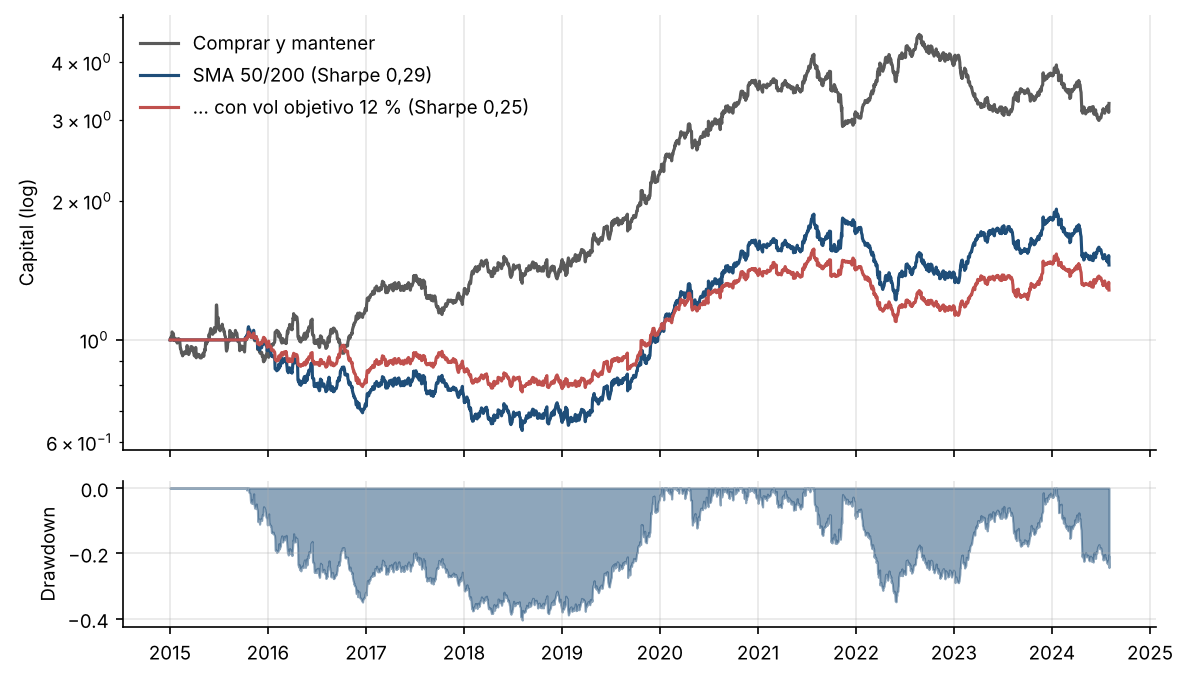
\includegraphics[width=0.95\textwidth]{f05_backtest}
\caption{Cruce de medias 50/200 sobre datos sintéticos, con y sin volatility targeting, y su drawdown.
En un activo con deriva positiva, el seguimiento de tendencia suele quedarse por detrás de comprar y
mantener: lo que aporta es reducir los drawdowns largos, no batir al activo.}
\end{figure}

\section{Los sesgos que destruyen backtests}
\begin{description}
\item[Look-ahead.] Usar información que no se tenía: cierres para decidir en la apertura del mismo día,
  datos fundamentales antes de su publicación, máximos del día en curso.
\item[Supervivencia.] Probar solo con las acciones que existen hoy olvida las que quebraron.
\item[Costes irreales.] Ignorar spread, comisiones, impacto, préstamo de títulos para cortos o el coste
  de financiación del apalancamiento.
\item[Sobreajuste (data snooping).] Probar muchas variantes y quedarse con la mejor.
\end{description}

\section{Sobreajuste: el sesgo de selección}\label{sec:sobreajuste}
Si pruebas $N$ configuraciones \emph{sin ventaja alguna}, el mejor Sharpe in-sample crece como
\begin{equation}
\E[\max_N \widehat{SR}] \approx \sigma_{SR}\Big[(1-\gamma)\Phi^{-1}\!\big(1-\tfrac1N\big)+\gamma\,\Phi^{-1}\!\big(1-\tfrac{1}{Ne}\big)\Big],
\end{equation}
con $\gamma\approx0{,}5772$ (\py{performance.expected\_max\_sharpe}). Con 3 años de datos
($\sigma_{SR}\approx 1/\sqrt{3}$), probar 100 variantes produce un «Sharpe 1,5» de puro ruido
(figura~\ref{fig:sobreajuste}).
\begin{figure}[h]\centering
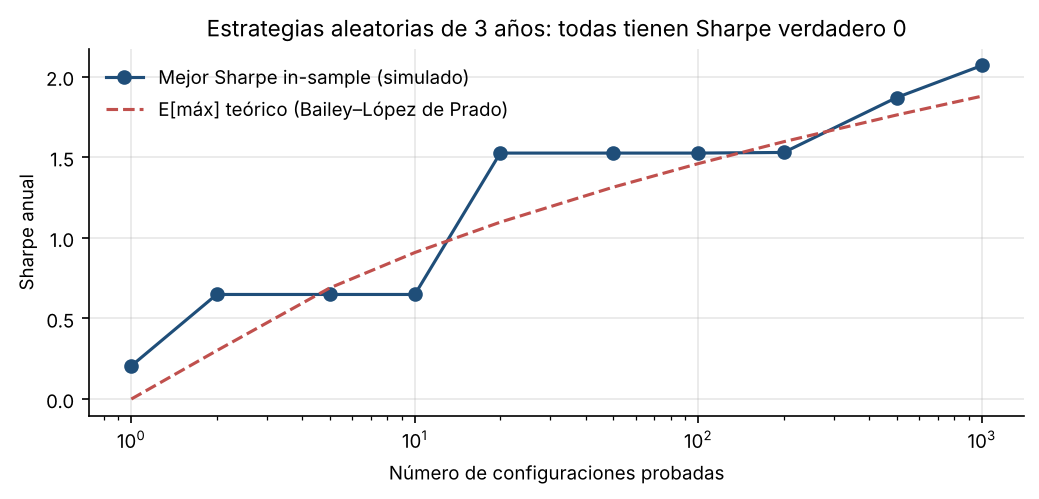
\includegraphics[width=0.85\textwidth]{f06_sobreajuste}
\caption{El mejor Sharpe de $N$ estrategias aleatorias. Si no cuentas cuántas pruebas hiciste, no sabes
lo que vale tu mejor resultado.}\label{fig:sobreajuste}
\end{figure}

\begin{practica}[Protocolo mínimo]
\begin{enumerate}
\item Escribe la hipótesis económica \emph{antes} de mirar los datos: ¿quién pierde el dinero que vas a ganar y por qué?
\item Reserva un tramo final de datos que no tocarás hasta el final (\emph{hold-out}).
\item Usa pocos parámetros y valores redondos; comprueba que los vecinos del óptimo también funcionan (meseta, no pico).
\item Valida en \emph{walk-forward} (\py{backtest.walk\_forward\_splits}): optimiza en una ventana, prueba en la siguiente.
\item Duplica los costes. Prueba en otros activos y otros periodos.
\item Anota cuántas variantes probaste y exige un Sharpe por encima del máximo esperado por azar.
\item Opera primero en papel o con tamaño mínimo y compara con el backtest.
\end{enumerate}
\end{practica}

\begin{ejercicios}
\begin{enumerate}
\item Con \py{scripts/backtest.py} prueba todas las combinaciones de \py{--rapida} 10, 20, 50 y \py{--lenta} 100, 150, 200. Anota el mejor Sharpe y compáralo con \py{expected\_max\_sharpe(9, ...)}.
\item Introduce a propósito un look-ahead (quita el \py{shift(1)} en una copia de \py{backtest}) y observa cómo «mejora» el resultado.
\end{enumerate}
\end{ejercicios}
